\chapter{Metodologia}
\label{chap:metodologia}

Neste capítulo, após o embasamento teórico sobre algumas técnicas introduzidas no decorrer do Capítulo \ref{cap:fundamentacao-teorica}, o problema é levantado na Seção \ref{sec:problema}. Além disso, na Seção \ref{sec:abordagem}, por meio das ideias apresentadas na Seção \ref{sec:deformacao} e no Capítulo \ref{cap:trabalhos-correlatos}, também será analisada uma abordagem para resolução do problema em questão.

\section{Problema}
\label{sec:problema}

Como ilustrado nas Figuras \ref{fig:domo_castelo}(a) e \ref{fig:domo_castelo}(b), muitas estruturas não retangulares comuns também possuem repetição, neste caso, o arranjo de janelas, blocos e pilares em paredes, torres e domos. Entretanto, uma \textit{shape grammar} baseada em uma caixa padrão não permite a geração de formas nem arranjos arredondados. Apesar de já existirem métodos para modelar ou aproximar formas curvadas ou deformadas, eles ainda apresentam problemas ou falham quando o assunto é a modelagem de formas mais complexas \cite{edelsbrunner2017}. Portanto, se os modelos exigem \textit{designs} curvados, sua criação é trabalhosa, pois as estruturas devem ser aproximadas por geometria plana ou ser colocadas, apropriadamente, com base em objetos pré-modelados \cite{zmugg2014}.

\begin{figure}[h!]
	\centering
	\captionsetup{width=15cm}
	\Caption{\label{fig:domo_castelo} Exemplo arquitetural de um domo e de uma torre de castelo.}	
	\UFCfig{}{
		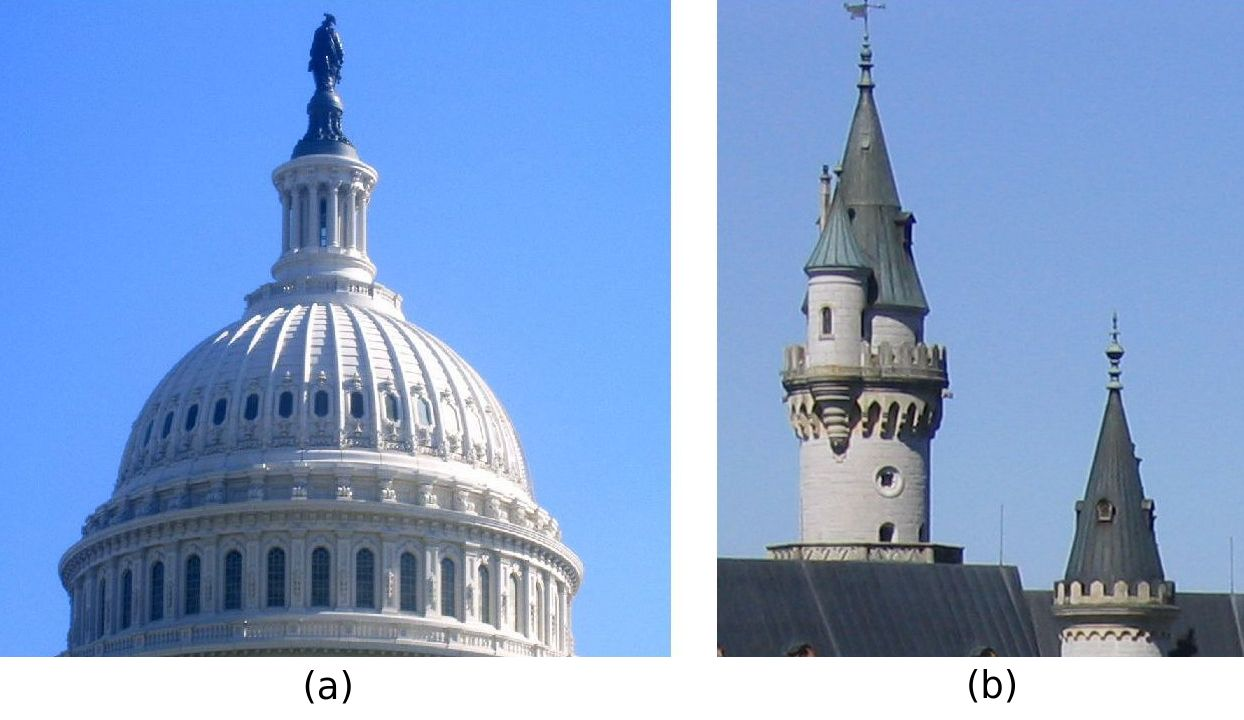
\includegraphics[width=15cm]{figuras/dome_castle.jpg}
	}
	{\Fonte{Adaptado de (a) \citeonline{renee} e (b) \citeonline{susan}}}	
\end{figure}

Conforme mencionado por \citeonline{wonka2018}, uma das limitações de implementação da \gls{SELEX} é justamente a incapacidade de modelar estruturas arredondadas diretamente, trabalhando apenas por meio de sua importação, como complementos, o que impossibilita a modelagem de fachadas curvadas, como a da Figura \ref{fig:selex_limitation}. Assim, na próxima seção, é discutida uma abordagem para resolução deste problema.

\begin{figure}[h!]
	\centering
	\captionsetup{width=15cm}
	\Caption{\label{fig:selex_limitation} Exemplo que está além da capacidade de modelagem da \gls{SELEX}.}	
	\UFCfig{}{
		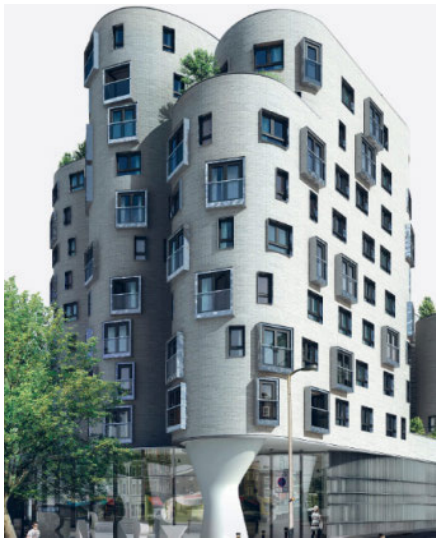
\includegraphics[width=7cm]{figuras/selex_facade_limitation.png}
	}
	{\Fonte{\cite{wonka2018}}}	
\end{figure}

\section{Abordagem}
\label{sec:abordagem}

A abordagem a ser desenvolvida se dará por meio de etapas bem definidas. A Seção \ref{sec:implementação}, explica o processo de implementação e integração da \gls{SELEX} com o \textit{software} de modelagem 3D. Logo após, na Seção \ref{sec:representacao_operacao}, são estudadas estratégias para representação das formas e execução das operações. Por fim, na Seção \ref{sec:aplicacao}, são analisadas algumas técnicas de deformação, bem como sua aplicabilidade ao contexto do problema.

\subsection{Implementação e integração}
\label{sec:implementação}

A implementação do interpretador para a \gls{SELEX} se dará por meio da utilização da biblioteca Python \textit{pyparsing}, desenvolvida por \citeonline{pyparsing}, que fornece uma abordagem alternativa para criar e executar gramáticas simples, cujo resultado é uma árvore sintática, conforme descrito nas especificações do material suplementar disponibilizado por \citeonline{wonka2018}.

Com base nesta árvore sintática, o próximo passo é a implementação dos \textit{scripts} para integração com o \textit{software} de modelagem Blender (versão 2.83), mantido pela \citeonline{blender}. 

Inicialmente, a modelagem se dará por meio da utilização das bibliotecas \textit{bpy} e \textit{bmesh}, ambas escritas em Python. Mais especificamente, o \gls{BPY}, mantido pela \citeonline{bpy}, é um módulo que contém vários submódulos com os quais se pode, por exemplo, adicionar objetos à cena 3D. Também mantido pela \citeonline{bmesh}, o \textit{BMesh}, por sua vez, é um módulo que fornece acesso às estruturas de dados dos objetos, como vértices, faces, arestas etc., e a alguns métodos de edição, como subdivisão, extrusão etc.

\subsection{Representação das formas e operações}
\label{sec:representacao_operacao}

As formas de construção, descritas na Seção \ref{sec:selex_definicao_formas}, poderão ser representadas pelos objetos padrões presentes no Blender, como plano e cubo. Cada objeto possui um conjunto de estruturas de dados que guardam informações sobre a sua representação, tais como quantidade de faces, arestas, vértices etc., bem como seus identificadores. Por meio destes atributos, será possível realizar a seleção de determinadas células (faces) ou grupo de células, para que operações possam ser aplicadas à elas, tais como \textit{groupCols()} ou \textit{groupRegions()}, conforme apresentado na Figura \ref{fig:seletores}. 

Um exemplo prévio do resultado da Figura \ref{fig:seletores}(a), mas gerado no Blender por meio do Código-fonte \ref{cod:group_exemplo}, é mostrado na Figura \ref{fig:blender_facade_previa}(a). Posteriormente, após a implementação das funções de seleção e agrupamento de faces, o resultado esperado é o das Figuras \ref{fig:blender_facade_previa}(b) e \ref{fig:blender_facade_previa}(c).

\begin{figure}[h!]
	\centering
	\captionsetup{width=15cm}
	\Caption{\label{fig:blender_facade_previa} Exemplo prévio de subdivisão por meio da utilização de \textit{scripts} no Blender.}	
	\UFCfig{}{
		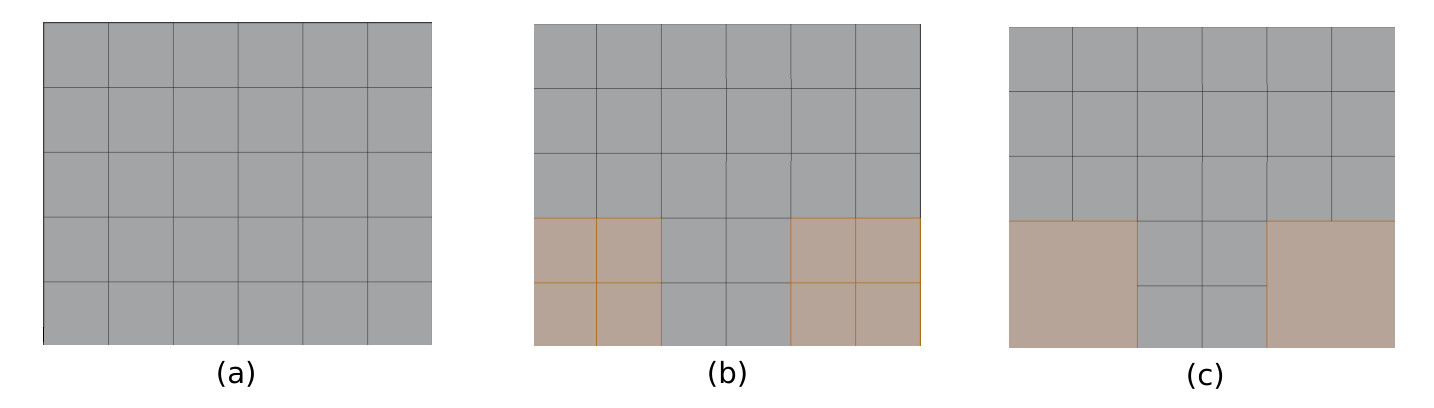
\includegraphics[width=15cm]{figuras/blender_facade.png}
	}
	{\Fonte{Próprio autor}}	
\end{figure}

Neste contexto, um ponto importante de definição é a representação das formas virtuais, uma vez que elas ditam como são realizadas as subdivisões, a fim de se adicionar janelas e portas, ou modificar a geometria do modelo, por exemplo. Intuitivamente, as formas virtuais podem ser representadas por matrizes, onde cada um de seus elementos representaria uma célula da grade. Isso seria bastante viável na definição atual, pois as formas virtuais são aplicadas em construções planas, como fachadas retas. Contudo, é importante ressaltar que, para sua utilização em superfícies curvadas, após uma possível operação de deformação, pode ser necessário o desenvolvimento de alguma outra estratégia.

\subsection{Aplicação de deformação nos modelos}
\label{sec:aplicacao}

O Blender dispõe de múltiplos recursos para manipulação de vértices, faces e arestas, em relação a diferentes eixos, conforme mostrado na Figura \ref{fig:blender_coordinates}, portanto, pretende-se utilizá-los na implementação das devidas estratégias para aplicar deformações nos modelos, a fim de se gerar arquiteturas arredondadas.

\begin{figure}[h!]
	\centering
	\captionsetup{width=15cm}
	\Caption{\label{fig:blender_coordinates} Representação do sistema de coordenadas do Blender: (a) eixos, (b) vértice, (c) aresta, (d) face.}	
	\UFCfig{}{
		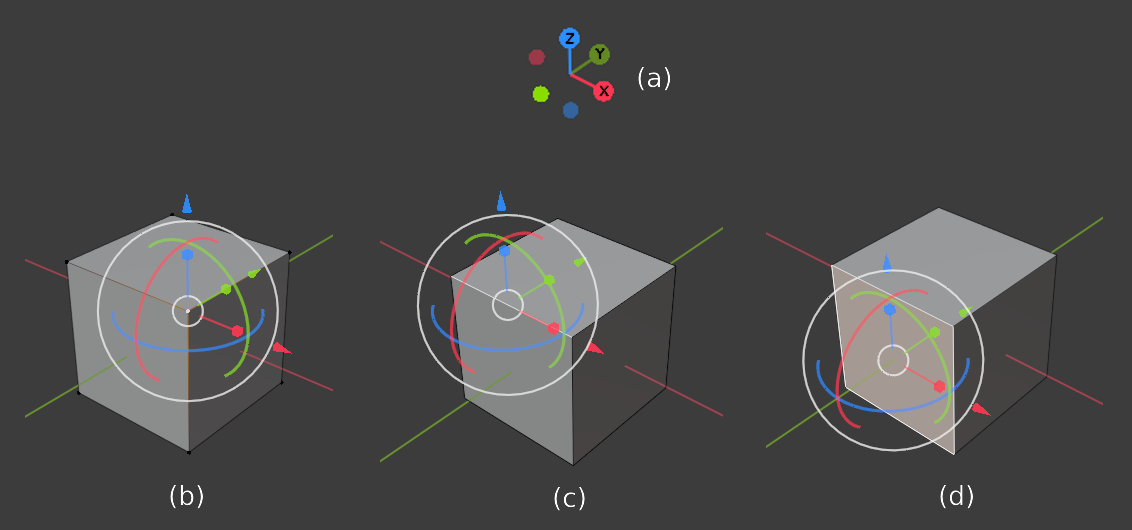
\includegraphics[width=15cm]{figuras/blender_coordinates.png}
	}
	{\Fonte{Próprio autor}}	
\end{figure}

Desconsiderando a questão em aberto sobre as formas virtuais, a ideia consiste na criação de uma nova operação para a \gls{SELEX}, que irá realizar uma deformação baseada em alguns parâmetros recebidos. Por exemplo, seja a operação \textit{roundShape}, que recebe por parâmetro o tipo de deformação (\textit{roundLeft}, \textit{roundRight}, \textit{roundTop}, \textit{roundBottom} ou \textit{roundFront}), a direção (\textit{inside} ou \textit{outside}), o nome da forma que será deformada, e outros possíveis parâmetros convenientes a serem definidos, podendo ser exemplificada da seguinte maneira:

\newpage

\vspace{0.5cm}

\begin{enumerate}[label=(\roman*)]
  \item \label{itm:roundfront} \textit{roundShape("roundFront", "outside", "cube", ...)}
  \item \label{itm:roundtop} \textit{roundShape("roundTop", "outside", "cube", ...)}
  \item \label{itm:roundbottom} \textit{roundShape("roundBottom", "outside", "cube", ...)}
  \item \label{itm:roundleft} \textit{roundShape("roundLeft", "outside", "cube", ...)}
  \item \label{itm:roundright} \textit{roundShape("roundRight", "outside", "cube", ...)}
\end{enumerate}

\vspace{0.5cm}

Como resultado, espera-se que seja possível gerar cada uma das ilustrações da Figura \ref{fig:round_shapes_blender}. Neste caso, cada forma corresponde ao resultado da aplicação de cada um dos respectivos tipos de deformação, representados de \ref{itm:roundfront} a \ref{itm:roundright}, sendo geradas a partir da Figura \ref{fig:round_shapes_blender}(a).

\begin{figure}[h!]
	\centering
	\captionsetup{width=15cm}
	\Caption{\label{fig:round_shapes_blender} Exemplo de cada tipo de deformação: (a) Forma original, (b) \textit{roundFront}, (c) \textit{roundTop}, (d) \textit{roundBottom}, (e) \textit{roundLeft}, (f) \textit{roundRight}.}	
	\UFCfig{}{
		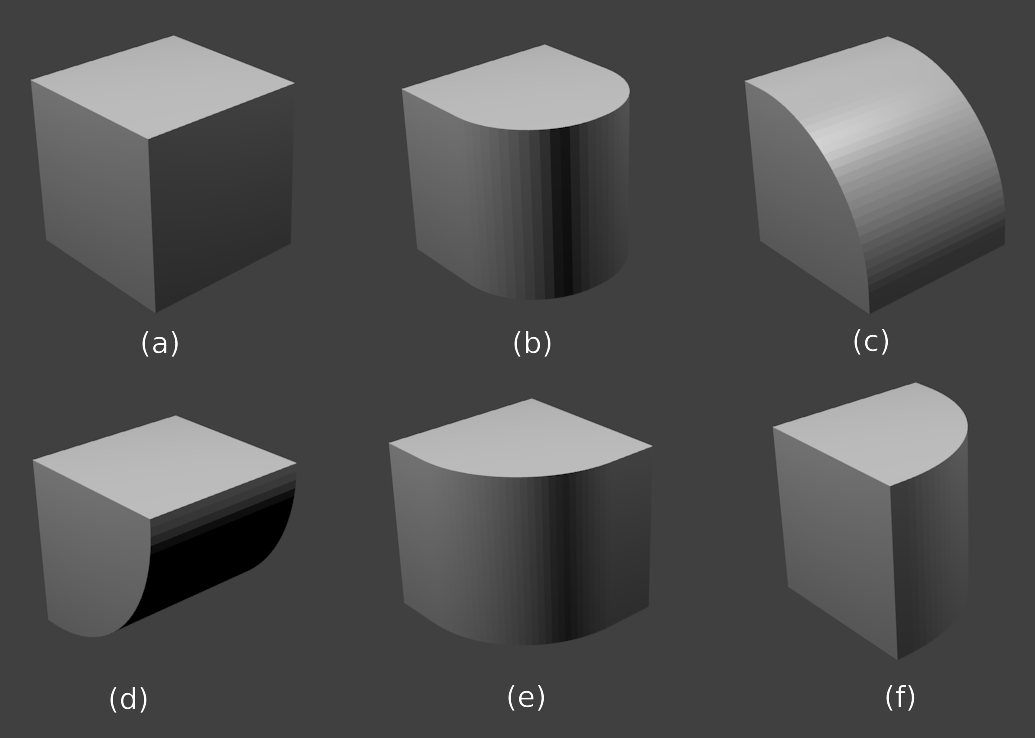
\includegraphics[width=13cm]{figuras/round_shapes.png}
	}
	{\Fonte{Próprio autor}}	
\end{figure}

Com viés experimental, os códigos-fonte \ref{cod:round_shapes_a_b}-\ref{cod:round_shapes_a_f}, foram implementados para criar uma deformação semelhante à cada uma das formas da Figura \ref{fig:round_shapes_blender}. No final, após a formalização da operação \textit{roundShape} e sua introdução na \gls{SELEX}, por meio da aplicação das devidas operações, espera-se que seja possível produzir arquiteturas com geometria arredondada, como apresentada na Figura \ref{fig:selex_limitation}, cuja modelagem inicial é mostrada na Figura \ref{fig:model_round_experimental}.

\begin{figure}[h!]
	\centering
	\captionsetup{width=15cm}
	\Caption{\label{fig:model_round_experimental} Modelagem inicial e experimental da arquitetura da Figura \ref{fig:selex_limitation}.}	
	\UFCfig{}{
		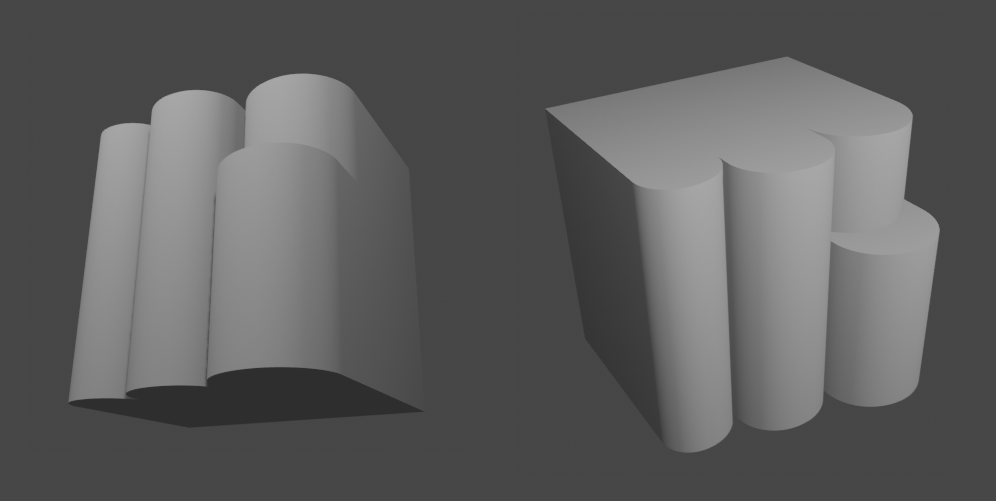
\includegraphics[width=15cm]{figuras/final_preview.png}
	}
	{\Fonte{Próprio autor}}	
\end{figure}

